\section{Classificazione non supervisionata}
Quando si esegue un training ti tipo gestito attraverso la Classificazione che è una tipologia di training non supervisionata. In questo caso le istanze di training non presentano etichetta e quindi la scelta del criterio di classificazione dipende dal modo di operare del learner.

Una possibilità è quella di raggruppare in base alla distanza (di Hamming, euclidea, per proiezioni..).

\begin{table}[H]
    \begin{center}
        \begin{tabular}{|l|l|}
            \hline
            \textbf{Classificazione supervisionata}       & \textbf{Classificazione non supervisionata}       \\ \hline
            Classi etichettate                   & Estrazione automatica delle classi       \\ \hline
            Struttura classificatoria conosciuta & Scarsa conoscenza dei dati da analizzare \\ \hline
        \end{tabular}
    \end{center}
\end{table}
Avere classi etichettate in fase di training è un costo che però fornisce un vantaggio in fase di classificazione. \\

Il sistema, nella classificazione non supervisionata, sceglie in completa autonomia quali classi formare; è possibile però scegliere il numero delle classi in cui suddividere i dati.
I sistemi non supervisionati sono utili quando la distribuzione dei valori degli attributi (feature) è in formazione utile/sufficiente per separare le istanze in più classi.

\subsection{Vantaggi apprendimento non supervisionato}
\begin{itemize}
    \item  Non è richiesta alcuna conoscenza a priori.
    \item  L’errore umano viene ridotto (analisi automatizzata).
    \item  Tutte le classi che hanno caratteristiche uniche vengono identificate.
    \item  Efficace con elementi di tipo numerico o di ordinamento intrinseco.
\end{itemize}
\subsection{Svantaggi apprendimento non supervisionato}
\begin{itemize}
    \item  Le classe ottenute non presentano necessariamente un significato.
    \item  Si ha un controllo limitato sulla procedura e sui risultati. 
    \item  Meno efficaci con elementi ordinati in modo arbitrario o poco netto.
\end{itemize}
\subsection{Clustering}
Il clustering è un procedimento che si pone come obiettivo la suddivisione di un insieme di elementi in sottoinsiemi accomunati da caratteristiche simili.
Si tratta della forma più semplice di apprendimento non supervisionato, con applicazioni in moltissimi campi.\\

\textbf{Dati necessari per il clustering}: 
\begin{itemize}
    \item  un insieme di elementi da classificare, ognuno specificato da un vettore caratteristico.
    \item  una misura di similarità (o di similarità) tra gli elementi
    \item  dei criteri da rispettare
        \begin{itemize}
            \item  \textbf{omogeneità}: elementi dello stesso cluster hanno un alto livello di similarità.
            \item  \textbf{separazione}: elementi di cluster diversi hanno un basso livello di similarità.
        \end{itemize}
\end{itemize}
Sia $N = \{e_1, \dots, e_n\}$ un insieme di $n$ elementi e sia $C = \{C_1, \dots, C_k\}$ una partizione di $N$ in sottoinsiemi. Ogni sottoinsieme è chiamato \textit{cluster} e $C$ è detto \textit{clustering} di $N$. \\
Due elementi $e_1$ e $e_2$ sono chiamati \textit{mates} rispetto a $C$ se sono membri dello stesso cluster in $C$. Inoltre un elemento può essere rappresentato da un vettore di numeri reali, ciascuno dei quali misura una specifica caratteristica (feature).

Misura di similarità come distanza tra vettori: 
\begin{itemize}
    \item \textbf{distanza euclidea}, questa distanza  è invariante rispetto a traslazioni e rotazioni degli assi, la notazione matematica è data da\[\displaystyle d(x,y) = \left[\sum_i (x_i - y_i)^2\right]^{\frac{1}{2}}\]
    \item \textbf{distanza di Manhattan}, in questo caso abbiamo che questa distanza non è invariante rispetto a traslazioni o rotazioni degli assi e pone meno enfasi sulle variabili con distanze maggiori, non elevando al quadrato le differenze. Questo se messa a confronto con la distanza euclidea. Per la notazione matematica abbiamo invece \[d(x,y) = \sum_i |x_i - y_i|\] 
    \item \textbf{distanza di Minkowski},il discorso in questo \[\displaystyle d(x,y) = \left[\sum_i |x_i - y_i|^k\right]^{\frac{1}{k}}\], dove $k$ è un intero positivo.
    \begin{itemize}
        \item Se $k=1$, si ha la distanza di Manhattan.
        \item Se $k=2$, si ha la distanza euclidea.
        \item Se $k=\infty$, si ha la distanza di Lagrange-Tchebychev.
\end{itemize}
\end{itemize}

\subsection{Tipologie di clustering}
\begin{figure}[H]
    \centering
    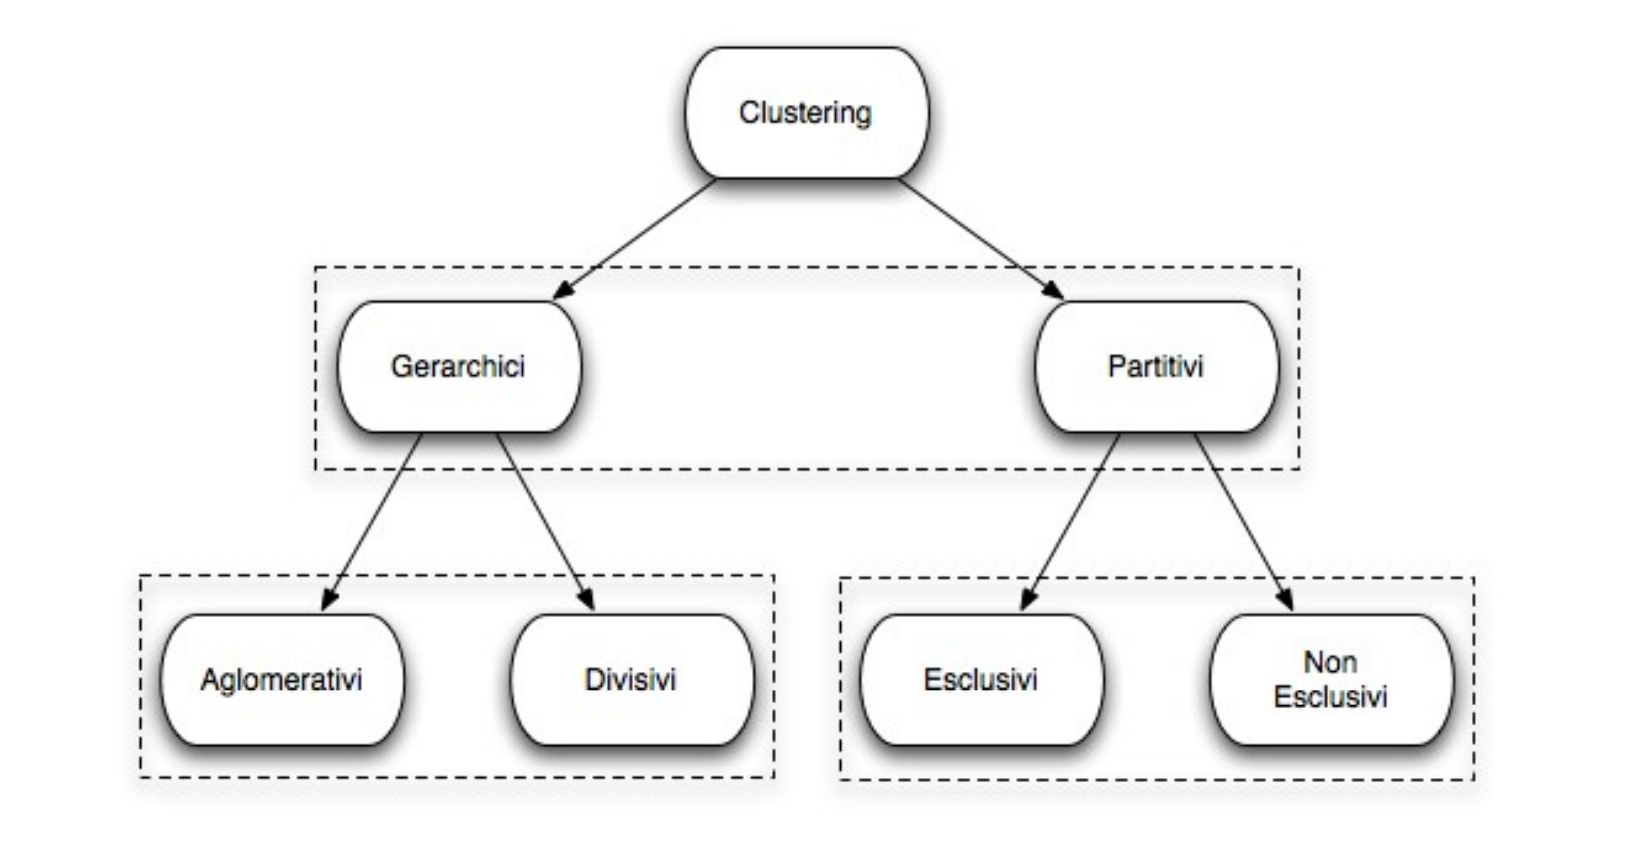
\includegraphics[scale = 0.3]{imm/cluster.PNG}
\end{figure}
Vediamo le due categorie principali esposte:
\begin{itemize}
    \item \textbf{Clustering gerarchico}, facendo questo tipo di clustering, quello che si va a eseguire, è il collocamento degli elementi in input in una struttura gerarchica ad albero, in cui le distanze tra nodi riflettono le similarità degli elementi. Gli elementi sono localizzati sulle foglie dell’albero.\\
    Ci sono alcuni vantaggi e svantaggi, infatti anche se sei si ha il vantaggio di avere una struttura singola, coerente e globale ed è un metodo intuitivo, purtroppo non ci sono esplicite partizioni nel cluster.
    \item \textbf{Clustering non gerarchico} mira a ripartire le $n$ unità della popolazione in $k$ gruppi, fornendo una sola partizione anziché una successione di partizioni tipica dei metodi gerarchici. Un esempio è il \textit{K-means}
\end{itemize}

\subsection{K-means}
Avevamo detto che è un metodo di cluster non gerarchico che opera per divisioni da un insieme iniziale. L'algoritmo prende in ingresso un intero $k$ e definisce iterativamente $k$ cluster che abbiano punti vicini in uno stesso cluster e punti distanti in cluster differenti. Si propone di minimizzare le distanze tra elementi e i centroidi dei clusters loro assegnati.
\subsubsection{Algoritmo K-means}(lavora solo con dati numerici)
Vediamo i vari step che vengono eseguiti durante l'utilizzo e l'implementazione di questo algoritmo:
\begin{enumerate}
    \item  Si fissano a caso $k$ centroidi iniziali di altrettanti cluster.
    \item  Per ogni individuo si calcola la distanza da ciascun centroide e lo si assegna al più vicino.
    \item  Per la partizione provvisoria così ottenuta si ricalcolano i centroidi di ogni cluster (media aritmetica).
    \item  Per ogni individuo si ricalcola la distanza dai centroidi e si effettuano gli eventuali spostamenti tra cluster.
    \item  Si ripetono le operazioni 3. e 4. finché si raggiunge il numero massimo di iterazioni impostate o non si verificano altri spostamenti.
\end{enumerate}
I vantaggi di questo algoritmo sono dati dal fatto che è di semplice implementazione e tempo di calcolo $\mathcal{O}(t\cdot k \cdot n)$ in cui $n$ è la cardinalità dell’insieme dei dati, $k$ è il numero di cluster e $t$ è il numero di iterazioni del ciclo (con $n \gg k, t$).\\
Si ha però una sensibilità rispetto alla scelta dei centroidi iniziali, non è possibile predire il numero di cluster non conoscendo i dati a priori, non esiste un $k$ ottimale e non ci sono proprietà che lo possano suggerire.\\
\subsubsection{Problematiche di K-means}
Con cluster con differenti dimensioni, con cluster con differenti densità, problematiche relative alle proprietà geometriche del cluster.
Una soluzione può essere l’utilizzo di un maggior numero di cluster a cui segue necessariamente una fase di unione in cluster più grandi.
\subsection{Misura di silhouette}
Data una distanza $d(i,j)$ tra due vettori o istanze $i,j$, in cluster con almeno due elementi al suo interno, è possibile calcolare:
\begin{itemize}
    \item \textbf{distanza media INTRA-cluster}: $a(i) = \displaystyle \frac{1}{|C_i| -1} \sum_{j \in C_i, i \neq j} d(i,j)$
    \item \textbf{distanza media INTER-cluster}: $b(i) = \displaystyle \min_{k \neq i} \frac{1}{|C_k|} \sum_{j \in C_k} d(i,j)$
    \item \textbf{silhouette} per un punto $i$: $s(i) = \displaystyle \frac{b(i) - a(i)}{\max \{a(i), b(i)\}}$\\
        Si vuole massimizzare la silhouette, massimizzando la distanza inter-cluster e minimizzando la distanza intra-cluster.
\end{itemize}
La media di $s(i)$, calcolata su tutti i punti di un cluster, è la misura di quanto strettamente sono raggruppati i punti nei cluster e quindi di quanto valido è il clustering effettuato.
infatti, in caso di troppi o troppo pochi cluster, come può accadere in seguito a una cattiva scelta di $k$ (numero di cluster), alcuni cluster avranno tipicamente una silhouette minore degli altri.
Quindi un plot delle silhouette potrebbe essere usato per determinare il numero di cluster da utilizzare per un determinato dataset.
